% 2010 年上海卷理科第 21 题：圆柱形灯笼、底面 8 等分与霓虹灯 A1B3、A3B5。
% 来源 PDF：普通高考/2010/2010上海理.pdf，SHA-256 e6181a8e02bfda976d5a2cee9432881769c184da4d3fca3b5a4d75c57a497ec6。
% 原页：第 2 页（A3 三栏）第 1 栏上部，书页码 628。
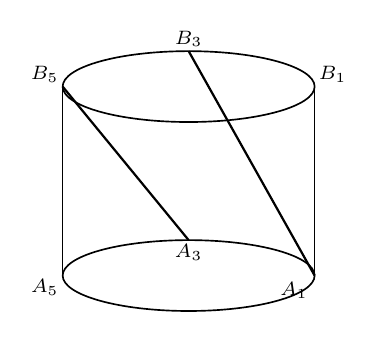
\begin{tikzpicture}[semithick, every node/.style={inner sep=1.2pt, font=\scriptsize}]
  % 下底与上口
  \draw (0,0) ellipse (1.6 and 0.45);
  \draw (0,2.4) ellipse (1.6 and 0.45);
  \draw (-1.6,0) -- (-1.6,2.4);
  \draw (1.6,0) -- (1.6,2.4);
  % 八个分点
  \foreach \a/\n in {0/1,45/2,90/3,135/4,180/5,225/6,270/7,315/8}{
    \coordinate (A\n) at ({1.6*cos(\a)},{0.45*sin(\a)});
    \coordinate (B\n) at ({1.6*cos(\a)},{2.4+0.45*sin(\a)});
  }
  % 霓虹灯
  \draw[thick] (A1) -- (B3);
  \draw[thick] (A3) -- (B5);
  % 标注关键点
  \node[below left=1pt] at (A1) {$A_1$};
  \node[below] at (A3) {$A_3$};
  \node[below left] at (A5) {$A_5$};
  \node[above] at (B3) {$B_3$};
  \node[above left] at (B5) {$B_5$};

  \node[above right] at (B1) {$B_1$};
\end{tikzpicture}
